\documentclass[11pt,a4paper]{article}
\usepackage[T1]{fontenc}
\usepackage{lmodern}
\usepackage[margin=25mm]{geometry}
\usepackage{amsmath}
\usepackage{booktabs,longtable}
\usepackage{graphicx}
\usepackage{xurl}
\usepackage[hidelinks]{hyperref}
\graphicspath{{../img/}{img/}}
\urlstyle{same}
\setlength{\parindent}{0pt}
\setlength{\parskip}{6pt}
\setlength{\emergencystretch}{3em}

\begin{document}
\begin{center}
    \Large\textbf{Bass Diffusion Analysis: Dreame X50 Ultra} \\[0.3cm]
    \large Nane Khachatryan \\[0.1cm]
    \normalsize DS 223: Marketing Analytics \\[0.1cm]
    \normalsize \today
\end{center}

\section*{1. Selected innovation}
I chose the Dreame X50 Ultra from TIME's Best Inventions of 2025 \cite{S01}:
\url{https://time.com/collections/best-inventions-2025/7318377/dreame-x50-ultra/}.
It is a robot vacuum and mop with retractable legs for crossing thresholds, a navigation sensor that lowers to fit under furniture, and a dock that automates maintenance \cite{S02}.

\section*{2. Similar innovation from the past}
My comparison is iRobot's Roomba, introduced in 2002, and its related home-cleaning robots \cite{S12}. Both Roomba and the X50 Ultra reduce the effort involved in cleaning floors through autonomous navigation and mechanical cleaning. The X50 adds improved obstacle crossing and access under furniture. Their purpose, technology, and household customers make iRobot's products a useful historical comparison. Including mopping robots also reflects the X50's combined vacuum-and-mop function.

The main difference is that iRobot's history covers several generations of products, while the X50 is one model in an established market. Its adoption might therefore move faster or end sooner. I use iRobot's shipments to estimate a possible diffusion pattern, while recognizing that shipments include replacements and do not count unique first-time customers.

\section*{3. Historical data}
The dataset contains 20 annual observations of worldwide iRobot home/consumer robot shipments, from FY2005 to FY2024. The figures come from the full-year columns in the company's financial-release tables, with a source for each observation below. The unit is thousands of robots, not revenue.

\begin{center}
\begin{tabular}{rrlrrl}
\toprule
Year & Shipments & Source & Year & Shipments & Source \\
\midrule
2005 & 663 & \cite{S05} & 2015 & 2,436 & \cite{S10} \\
2006 & 725 & \cite{S05} & 2016 & 2,943 & \cite{S11} \\
2007 & 899 & \cite{S06} & 2017 & 3,698 & \cite{S11} \\
2008 & 1,054 & \cite{S07} & 2018 & 4,537 & \cite{S12} \\
2009 & 988 & \cite{S07} & 2019 & 4,989 & \cite{S12} \\
2010 & 1,269 & \cite{S08} & 2020 & 5,494 & \cite{S13} \\
2011 & 1,371 & \cite{S08} & 2021 & 5,602 & \cite{S14} \\
2012 & 1,621 & \cite{S09} & 2022 & 4,182 & \cite{S14} \\
2013 & 1,933 & \cite{S09} & 2023 & 3,034 & \cite{S15} \\
2014 & 2,174 & \cite{S10} & 2024 & 2,463 & \cite{S16} \\
\bottomrule
\end{tabular}
\end{center}

The reports call the measure ``Home Robots,'' then ``Consumer units shipped,'' and later total robot units. Separately reported military robots are excluded. This is a broad home-robot series, not vacuum-only data. In FY2024, the product split changed to solo/other and 2-in-1 robots, but the total remains comparable at the portfolio level: both releases report 3.034 million for FY2023 \cite{S15,S16}. Product mix still changes over time.

The observed total is 52.075 million units. No missing year is filled with zero or interpolated. FY2024 is the historical cutoff for this retrospective analysis of a 2025 invention; it is not a claim that the data were all available on launch day.

\section*{4. Bass model parameters}
Let $F(t)$ be the cumulative fraction of the potential market that has adopted by time $t$. The Bass model uses an innovation coefficient $p$, an imitation coefficient $q$, and market potential $M$ \cite{S03}:
\[
F(t)=\frac{1-e^{-(p+q)t}}{1+(q/p)e^{-(p+q)t}},
\qquad f(t)=[p+qF(t)][1-F(t)].
\]
Here, $p$ represents adoption independent of previous adopters, while $q$ represents influence associated with previous adopters. The instantaneous adoption rate is $Mf(t)$. For yearly totals, I use its integral over each year:
\[
\widehat y_t=M\bigl[F(t)-F(t-1)\bigr].
\]
I estimate $p$, $q$, and $M$ by nonlinear least squares, minimizing $\sum_t(y_t-\widehat y_t)^2$ with positive parameters and equal weight for each observation. The code uses millions of robots. FY2002 is approximated as year 1, so FY2005 is year 4. The missing launch-period observations are excluded from fitting. Fiscal years are treated as equally spaced, ignoring small differences in their length.

\begin{center}
\begin{tabular}{lr}
\toprule
Parameter or measure & Estimate \\
\midrule
Innovation coefficient $p$ (per year) & 0.000881 \\
Imitation coefficient $q$ (per year) & 0.325893 \\
Analogue market potential $M$ & 59.97 million units \\
$R^2$ & 0.909 \\
Root mean squared error (RMSE) & 0.481 million units \\
\bottomrule
\end{tabular}
\end{center}

Since $q$ is much larger than $p$, the fitted curve relies mainly on imitation once adoption grows. This is a model interpretation, not proof of a causal word-of-mouth effect. The fitted $M$ represents eventual shipment volume for the analogue; it is not Dreame's market size or a count of distinct households.

\begin{center}\begin{minipage}{\linewidth}\centering
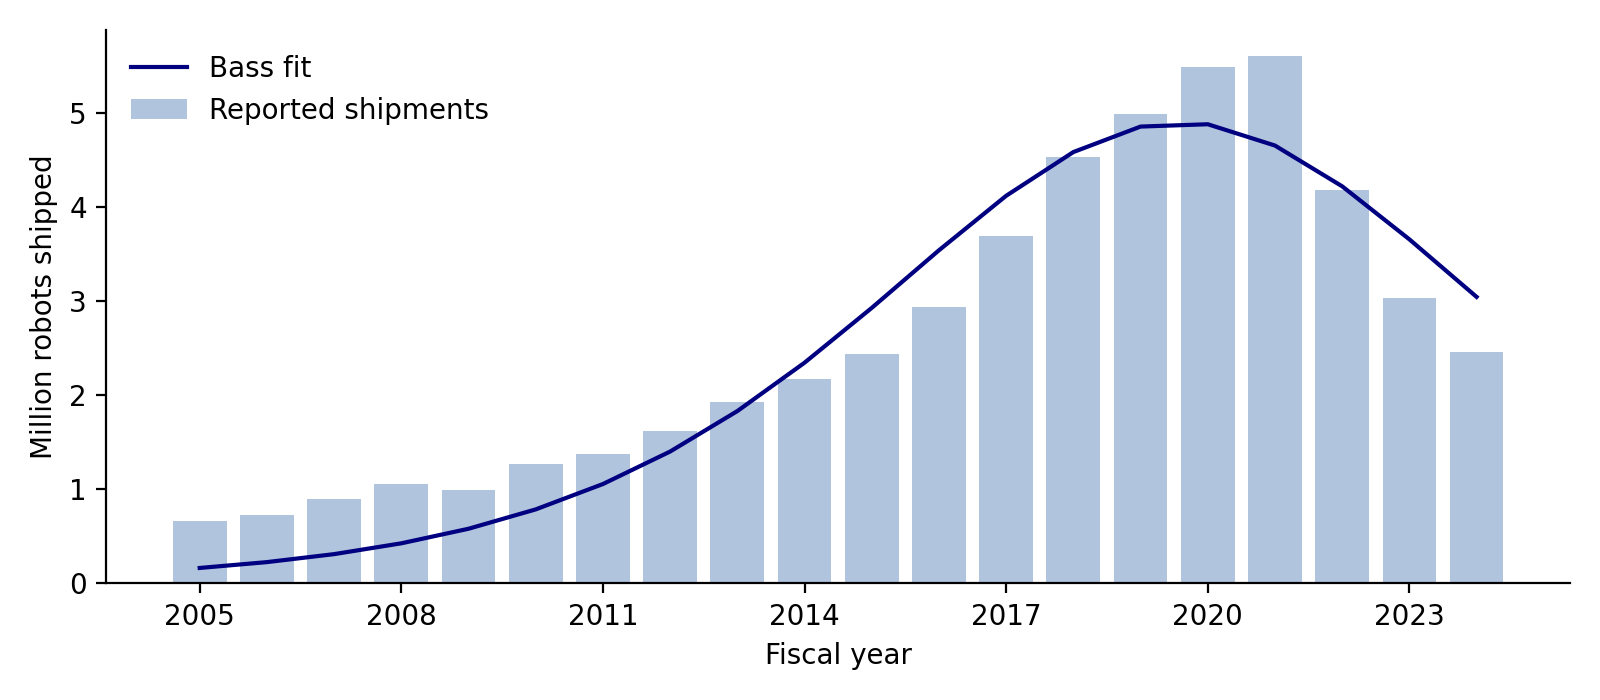
\includegraphics[width=0.90\linewidth]{historical_fit.png}

\small Figure 1. Reported iRobot shipments and fitted annual volumes.
\end{minipage}\end{center}

\textbf{Forecast check.} I also fit the model using only FY2005--FY2021 and predict the remaining three years:
\begin{center}
\begin{tabular}{rrrr}
\toprule
Fiscal year & Actual & Bass prediction & Last-value prediction \\
\midrule
2022 & 4.182 & 6.456 & 5.602 \\
2023 & 3.034 & 6.963 & 5.602 \\
2024 & 2.463 & 7.396 & 5.602 \\
\bottomrule
\end{tabular}
\end{center}
All values are millions of robots. The holdout RMSE is 3.871 million, compared with 2.481 million when simply repeating the 2021 value. The model fits the overall historical shape but fails to predict the decline, so the Dreame forecast below should be treated as an illustrative scenario.

\section*{5. Predicted diffusion of Dreame X50 Ultra}
I transfer the analogue's estimated $p$ and $q$ to the X50 Ultra:
\[
p_D=0.000881,\qquad q_D=0.325893.
\]
This assumes a similar diffusion pattern; these are not coefficients estimated from Dreame sales. Starting from $F(0)=0$, cumulative adoption is $M_DF(t)$ and adoption during year $t$ is $M_D[F(t)-F(t-1)]$. The market potential $M_D$ is estimated separately in section 7. A household can be a first-time X50 adopter even if it previously owned a different robot vacuum.

\begin{center}
\begin{tabular}{rrr}
\toprule
Year after launch & Cumulative adoption & Adoption during that year \\
\midrule
1 & 0.10\% & 0.10\% \\
3 & 0.45\% & 0.20\% \\
5 & 1.10\% & 0.38\% \\
10 & 6.37\% & 1.76\% \\
15 & 26.47\% & 5.90\% \\
20 & 64.98\% & 7.76\% \\
25 & 90.49\% & 3.21\% \\
30 & 97.99\% & 0.76\% \\
\bottomrule
\end{tabular}
\end{center}
Both columns are percentages of eventual potential X50 adopters, not percentages of all U.S. households or annual market share.

\begin{center}\begin{minipage}{\linewidth}\centering
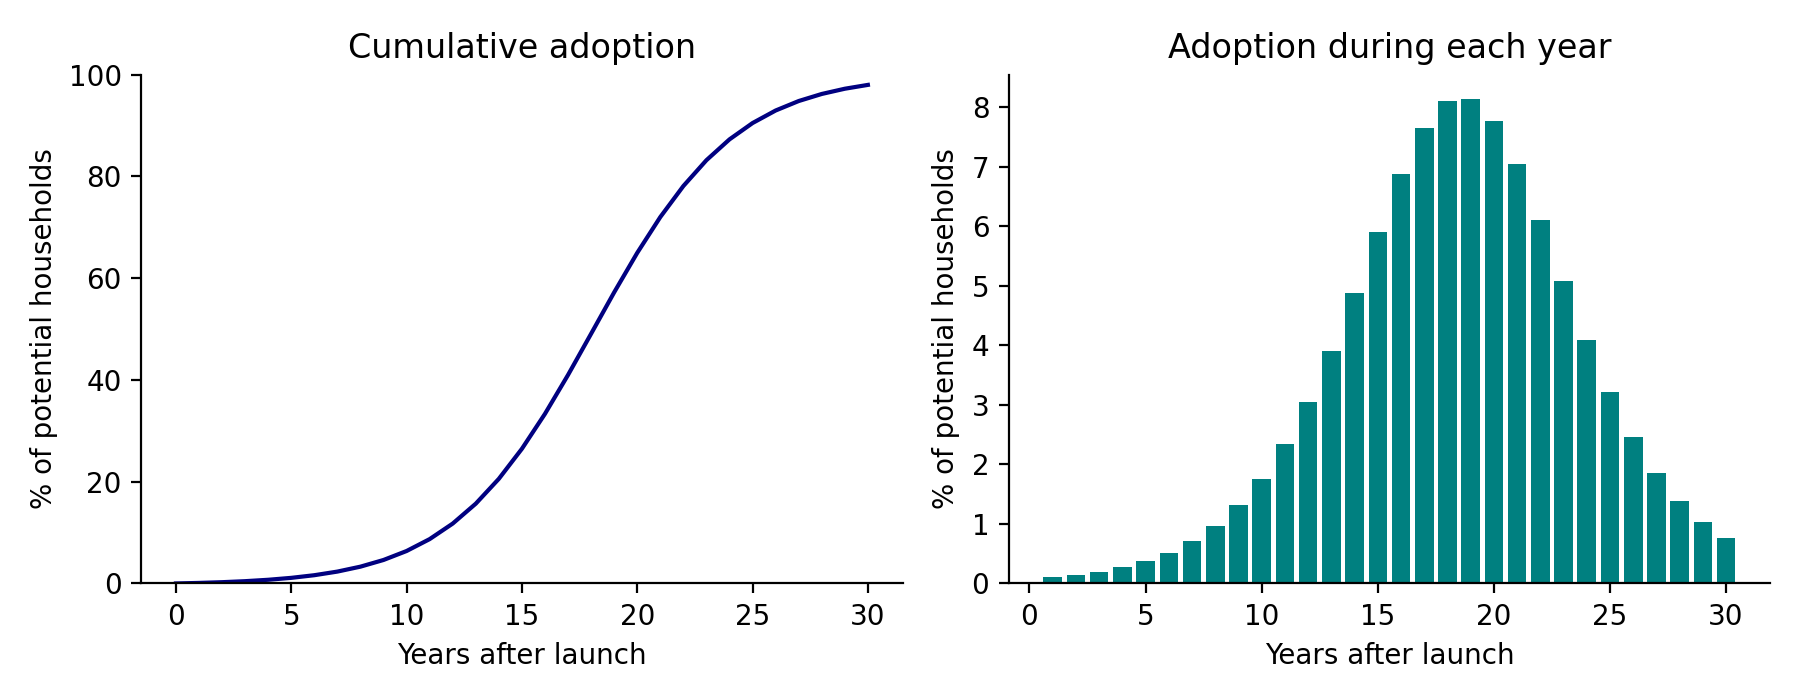
\includegraphics[width=0.85\linewidth]{normalized_forecast.png}

\small Figure 2. Predicted cumulative and annual adoption shares.
\end{minipage}\end{center}

The model predicts slow initial adoption, followed by growth and eventual saturation. Half of the potential market adopts after about 18.11 years. The continuous peak is
\[
t^*=\frac{\ln(q/p)}{p+q}=18.10\text{ years}.
\]
The largest one-year total occurs in year 19, at 8.14\% of the potential market. The 30-year horizon shows the full mathematical curve; it is not a realistic claim that this exact retail model will remain available for 30 years. The long peak time is a clear weakness of borrowing a category-building portfolio's adoption pattern for a newer model.

\section*{6. Geographic scope}
I use the United States because Dreame sells the X50 there and reliable household data are available. Dreame announced availability on its U.S. website and Amazon from February 14, 2025, at a launch price of \$1,699.99 \cite{S18}. The 2024 American Community Survey estimates 132,737,146 U.S. households \cite{S17}. Households are a more suitable unit than individuals for a shared home appliance.

The historical iRobot data are worldwide, while the Dreame forecast is U.S.-specific. Transferring $p$ and $q$ therefore also assumes that the worldwide pattern is useful for this country. I do not transfer the worldwide analogue's $M$ to the U.S. market.

\section*{7. Number of adopters by period}
There is no verified X50 household-adoption series in this project, so I use a Fermi estimate for market potential:
\[
M_D=H\times s\times c,
\]
where $H$ is the number of U.S. households, $s$ is the share that could consider a premium robot vacuum, and $c$ is the share of that segment that eventually chooses the X50.

The household count $H=132{,}737{,}146$ is sourced from the ACS \cite{S17}. The other inputs are explicitly assumptions, not reported statistics:
\begin{itemize}
\item I assume $s=20\%$, or one household in five. This restricts the market to a minority that might have the budget, interest, and suitable home for this premium appliance. The launch price motivates a restricted market but does not establish this exact percentage.
\item I assume $c=10\%$ in the base case, allowing for other brands and later models. Low and high cases use 5\% and 20\%. These values are judgment-based scenarios, not estimated brand shares.
\end{itemize}

For the base case,
\[
M_D=132{,}737{,}146\times0.20\times0.10
\approx 2{,}654{,}743\text{ households}.
\]

\begin{center}
\begin{tabular}{lrrr}
\toprule
Scenario & Segment captured & Share of all households & $M_D$ \\
\midrule
Low & 5\% & 1\% & 1,327,371 \\
Base & 10\% & 2\% & 2,654,743 \\
High & 20\% & 4\% & 5,309,486 \\
\bottomrule
\end{tabular}
\end{center}

These cases keep $p$ and $q$ fixed, so they change the size of adoption but not its timing. They are not confidence intervals and do not cover all uncertainty. For example, reducing the assumed premium segment from 20\% to 10\% would also halve the base forecast.

\begin{center}\begin{minipage}{\linewidth}\centering
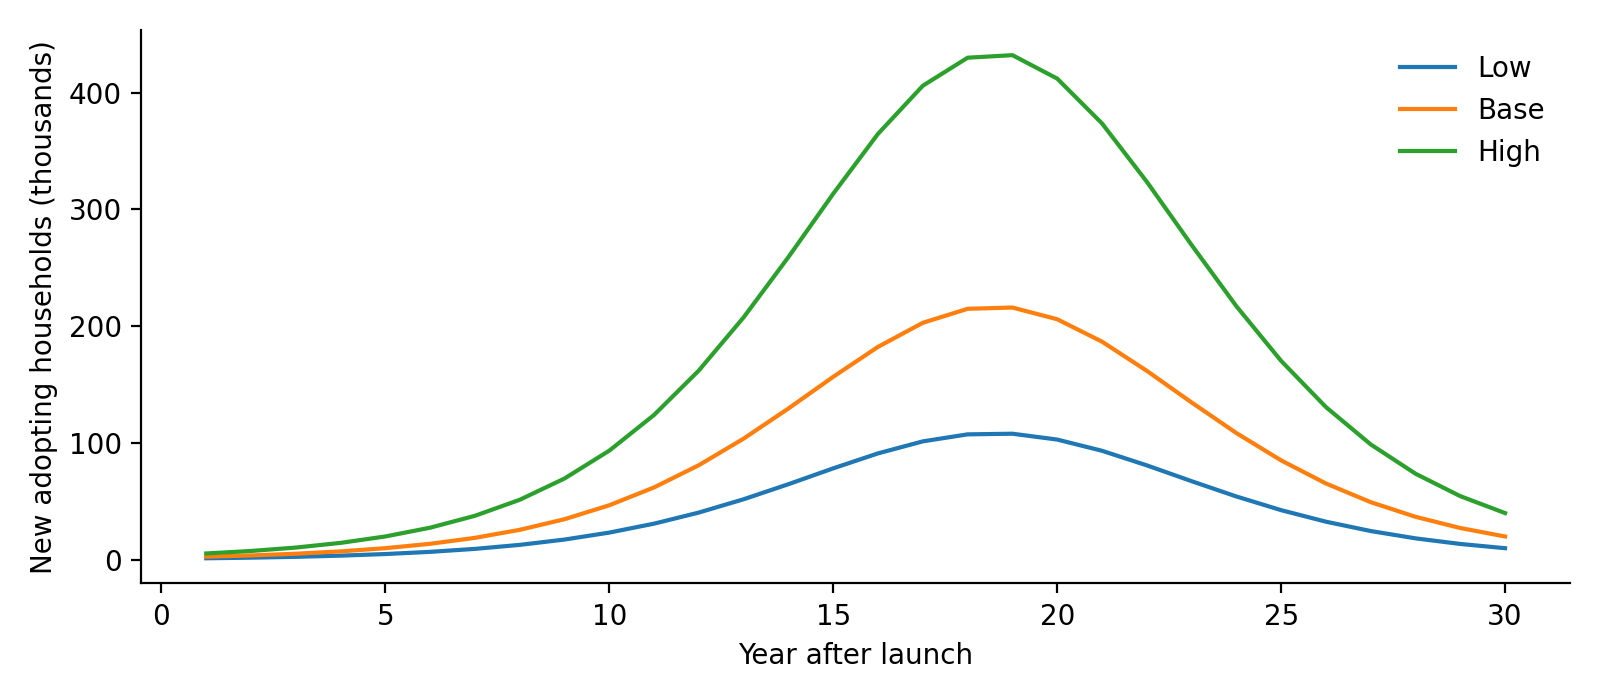
\includegraphics[width=0.95\linewidth]{us_adopters.png}

\small Figure 3. Annual U.S. household adoption under three market-size assumptions.
\end{minipage}\end{center}

Each period is a full year after launch: year 1 is approximately February 2025--February 2026, rather than calendar 2025. I calculate annual adopters as $M_D[F(t)-F(t-1)]$ and cumulative adopters as $M_DF(t)$. The following table shows all 30 modeled years. The base case gives about 2,763 new adopting households in year 1 and 46,775 in year 10. Cumulative adoption reaches about 169,211 households by year 10.

\newpage
\textbf{Forecast of U.S. adopting households}

{\small
\begin{longtable}{rrrrr}
\toprule
Year & Low: annual & Base: annual & High: annual & Base: cumulative \\
\midrule
\endfirsthead
\toprule
Year & Low: annual & Base: annual & High: annual & Base: cumulative \\
\midrule
\endhead
1 & 1,382 & 2,763 & 5,527 & 2,763 \\
2 & 1,911 & 3,822 & 7,643 & 6,585 \\
3 & 2,640 & 5,281 & 10,561 & 11,866 \\
4 & 3,643 & 7,287 & 14,573 & 19,152 \\
5 & 5,018 & 10,037 & 20,073 & 29,189 \\
6 & 6,895 & 13,790 & 27,580 & 42,979 \\
7 & 9,441 & 18,882 & 37,763 & 61,861 \\
8 & 12,866 & 25,732 & 51,464 & 87,593 \\
9 & 17,422 & 34,844 & 69,688 & 122,437 \\
10 & 23,387 & 46,775 & 93,549 & 169,211 \\
11 & 31,032 & 62,065 & 124,130 & 231,276 \\
12 & 40,548 & 81,096 & 162,192 & 312,372 \\
13 & 51,929 & 103,858 & 207,715 & 416,230 \\
14 & 64,821 & 129,643 & 259,286 & 545,873 \\
15 & 78,376 & 156,751 & 313,503 & 702,624 \\
16 & 91,192 & 182,384 & 364,767 & 885,008 \\
17 & 101,478 & 202,957 & 405,914 & 1,087,965 \\
18 & 107,474 & 214,948 & 429,896 & 1,302,913 \\
19 & 108,021 & 216,043 & 432,085 & 1,518,955 \\
20 & 103,010 & 206,019 & 412,039 & 1,724,975 \\
21 & 93,421 & 186,841 & 373,683 & 1,911,816 \\
22 & 80,945 & 161,890 & 323,779 & 2,073,706 \\
23 & 67,408 & 134,815 & 269,631 & 2,208,521 \\
24 & 54,305 & 108,610 & 217,220 & 2,317,131 \\
25 & 42,593 & 85,186 & 170,372 & 2,402,317 \\
26 & 32,711 & 65,421 & 130,843 & 2,467,739 \\
27 & 24,717 & 49,434 & 98,868 & 2,517,173 \\
28 & 18,449 & 36,898 & 73,796 & 2,554,071 \\
29 & 13,645 & 27,289 & 54,578 & 2,581,360 \\
30 & 10,023 & 20,046 & 40,092 & 2,601,406 \\
\bottomrule
\end{longtable}
}
Counts are rounded to the nearest household, so rounded annual values may not sum exactly to rounded cumulative values. The CSV also contains cumulative forecasts for the low and high scenarios.

\textbf{Interpretation and limitations.} The base forecast peaks at about 216,043 new adopting households in year 19. These estimates depend on the assumed market size, a fixed household population, and unchanged diffusion coefficients. The source data include repeat purchases, retailer inventory, and several product generations. They are not direct observations of first-time household adoption. Competition can also cause iRobot's decline without the entire market being saturated.

Most importantly, this single-product forecast borrows a much longer portfolio history. The poor holdout forecast and long predicted peak mean the result is useful as a Bass-model exercise, but not as a precise commercial sales forecast. Product-specific first-purchase data would be needed to improve it.

\clearpage
\begin{thebibliography}{S18}
\bibitem[S01]{S01} TIME (2025). Dreame X50 Ultra: The Best Inventions of 2025.
\url{https://time.com/collections/best-inventions-2025/7318377/dreame-x50-ultra/}

\bibitem[S02]{S02} Dreame (n.d.). X50 Ultra product specifications and U.S. product listing.
\url{https://www.dreametech.com/products/x50-ultra-robot-vacuum}

\bibitem[S03]{S03} Bass, F. M. (1969). A new product growth for model consumer durables. Management Science, 15(5), 215-227.
\url{https://doi.org/10.1287/mnsc.15.5.215}

\bibitem[S05]{S05} iRobot Corporation (2007-02-12). Fourth-quarter and full-year 2006 results. Supplemental Information: Home Robots units shipped, full-year columns.
\url{https://www.sec.gov/Archives/edgar/data/1159167/000095013507000702/b64144irexv99w1.htm}

\bibitem[S06]{S06} iRobot Corporation (2008-02-19). Fourth-quarter and full-year 2007 results. Supplemental Information: Home Robots units shipped, full-year columns.
\url{https://www.sec.gov/Archives/edgar/data/1159167/000095013508001079/b68626irexv99w1.htm}

\bibitem[S07]{S07} iRobot Corporation (2010). Fourth-quarter and full-year 2009 results. Supplemental Information: Home Robots units shipped, full-year columns.
\url{https://media.irobot.com/press-releases?item=122487}

\bibitem[S08]{S08} iRobot Corporation (2012-02-08). Fourth-quarter and full-year 2011 results. Supplemental Information: Home Robots units shipped, full-year columns.
\url{https://media.irobot.com/press-releases?item=122437}

\bibitem[S09]{S09} iRobot Corporation (2014-02-05). Fourth-quarter and full-year financial results (FY2013). Supplemental Information: Home Robots units shipped.
\url{https://media.irobot.com/2014-02-05-iRobot-Reports-Fourth-Quarter-and-Full-Year-Financial-Results}

\bibitem[S10]{S10} iRobot Corporation (2016-02-10). Fourth-quarter and full-year financial results (FY2015). Supplemental Information: Home Robots units shipped.
\url{https://media.irobot.com/2016-02-10-iRobot-Reports-Fourth-Quarter-and-Full-Year-Financial-Results}

\bibitem[S11]{S11} iRobot Corporation (2018-02-07). Record fourth-quarter and full-year revenue (FY2017). Supplemental Information: consumer units shipped and vacuum units.
\url{https://media.irobot.com/2018-02-07-iRobot-Reports-Record-Fourth-Quarter-and-Full-Year-Revenue}

\bibitem[S12]{S12} iRobot Corporation (2020-02-05). Fourth-quarter and full-year 2019 financial results. Supplemental Information: FY2018 and FY2019 units shipped. Company description dates Roomba introduction to 2002.
\url{https://media.irobot.com/2020-02-05-iRobot-Reports-Fourth-Quarter-and-Full-Year-2019-Financial-Results}

\bibitem[S13]{S13} iRobot Corporation (2021-02-10). Fourth-quarter and full-year 2020 financial results. Supplemental Information: units shipped.
\url{https://media.irobot.com/2021-02-10-iRobot-Reports-Fourth-Quarter-and-Full-Year-2020-Financial-Results}

\bibitem[S14]{S14} iRobot Corporation (2023-02-13). Fourth-quarter and full-year 2022 financial results. Supplemental Information: robot units shipped, FY2021 and FY2022.
\url{https://media.irobot.com/2023-02-13-iRobot-Reports-Fourth-Quarter-and-Full-Year-2022-Financial-Results}

\bibitem[S15]{S15} iRobot Corporation (2024-02-26). Fourth-quarter and full-year 2023 financial results. Supplemental Information: robot units shipped.
\url{https://media.irobot.com/2024-02-26-iRobot-Reports-Fourth-Quarter-and-Full-Year-2023-Financial-Results}

\bibitem[S16]{S16} iRobot Corporation (2025-03-12). Fourth-quarter and full-year 2024 financial results. Supplemental Information: total robot units shipped; solo/other and 2-in-1 categories.
\url{https://media.irobot.com/2025-03-12-iRobot-Reports-Fourth-Quarter-and-Full-Year-2024-Financial-Results}

\bibitem[S17]{S17} U.S. Census Bureau (2024). American Community Survey 1-Year Estimates Subject Table S1101: Households and Families. Total U.S. households: 132,737,146.
\url{https://data.census.gov/table/ACSST1Y2024.S1101}

\bibitem[S18]{S18} Dreame Technology (2025-01-06). All Dreams in One Dreame: Dreame Technology Unveils Next-Generation Smart Home Ecosystem at CES 2025. Press release.
\url{https://www.prnewswire.com/news-releases/all-dreams-in-one-dreame-dreame-technology-unveils-next-generation-smart-home-ecosystem-at-ces-2025-302342783.html}

\end{thebibliography}
\end{document}
